\documentclass{article}

% Language setting
% Replace `english' with e.g. `spanish' to change the document language
\usepackage[french]{babel}
\usepackage[fleqn]{amsmath} % Aligner les équations à gauche


% Set page size and margins
% Replace `letterpaper' with`a4paper' for UK/EU standard size
\usepackage[letterpaper,top=2cm,bottom=2cm,left=3cm,right=3cm,marginparwidth=1.75cm]{geometry}

% Useful packages

\usepackage{amsmath}
\usepackage{graphicx}
\usepackage{subcaption}
\usepackage[colorlinks=true, allcolors=blue]{hyperref}

\title{TD 12}
\author{IPESUP - PC }
\date{7/02/2024}

\begin{document}
\maketitle



\section{Onde dans un tuyau}




\begin{enumerate}
  \item 
  Avec un instrument à vent, lorsque l' instrumentiste joue des notes montant vers les aigus, le
  rapport de la longueur d'onde au diamètre du tuyau décroît et des ondes non planes peuvent
  se propager. Les ondes satisfont à une équation de propagation tridimensionnelle :
  
  $\Delta p(M,t)-{\frac{1}{c^{2}}}{\frac{\partial^{2}p}{\partial t^{2}}}(M,t)=0\,.$
  
  
  \begin{figure}[h]
    \centering
    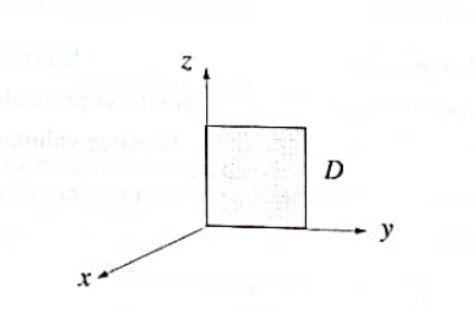
\includegraphics[width=0.4\textwidth]{tuyau_schéma.png}
    \label{fig:maison}
      \caption{}
  \end{figure}
    Justifier la forme ${{{p(z,y,z,t)}}}\,=Y(y)Z(z){\exp}{{\big(}i(k x-\omega t){\big)}}$ sous laquelle on va rechercher des
  solutions de l’équation d’onde.
  \item Quelle est la condition imposée à la vitesse du fluide sur les parois ? En déduire les conditions
  imposées aux fonctions $Y(y)$ et$ Z(z)$.

  \item Démontrer que la pulsation $\omega$ et le nombre d'onde $k$ sont liés à la dimension transversale
  $D$ du tuyau par :

  $\omega^{2}=k^{2}c^{2}+{\frac{\pi^{2}c^{2}}{D^{2}}}\left(a^{2}+b^{2}\right)$, $a$ et $b$ étant des entiers naturels.
  \item Les répartitions de $Y(y)Z(z)$ de l'amplitude de la surpression dans la section droite sont
  appelées modes transverses du tuyau et caractérisés par le couple ${a,b}$. À quel couple correspond la propagation d’une onde plane ?





  \item Exprimer la relation précédente  sous la forme ${\frac{f}{f_{c}}}=f(\{a,b\},k D)$ dans laquelle $f_c=\frac{c}{2D}$
  Pourquoi appelle-t-on $f_c$, fréquence de coupure ?
  Le tracé sur la fig. \ref{fig:graphe} représente les courbes des premiers modes $\{0,0\}, \{1,0\}, \{0,1\}$ et $\{1,1\}$.
  Associer à chacune de ces courbes le mode correspondant.


  
  
  \begin{figure}[h]
    \centering
    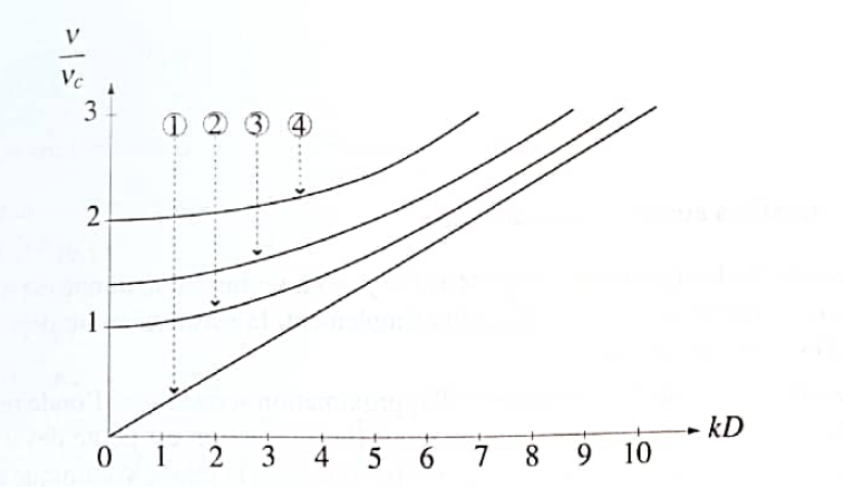
\includegraphics[width=0.4\textwidth]{graphe.png}
    \caption{}

    \label{fig:graphe}
  \end{figure}


  % symbole pour { :
  % \{

  


  \item Les instruments réels à section constante sont cylindriques, de rayon $a$. L’étude se fait de
  la même façon que pour un tuyau à section carrée mais le résultat fait intervenir d’autres fonctions. 
  La fréquence de coupure la plus basse est alors : $\scriptstyle f_{c}={\frac{1.84c}{2\pi a}}.$
  \begin {itemize}

    \item Effectuer l’application numérique pour un tuyau de rayon $a = 1 cm$. L'hypothèse d’une
   onde plane seule dans le tuyau est-elle plausible ?
    \item On réalise I'expérience suivante : un émetteur d’ultrasons envoie des trains d’onde de fréquence
    $f_e = 40,0 kHz$, de durée $\Delta t = 500 \mu s$, dans un tuyau cylindrique de diamètre $35,0 mm$.
    Un récepteur est placé à l’autre extrémité du tuyau, sur l’axe de celui-ci, face à l’émetteur.
    La distance entre l’émetteur et le récepteur est $L = 201 cm$. On observe à l’oscilloscope les signaux suivants :


    \begin{figure}[h]
      \centering
      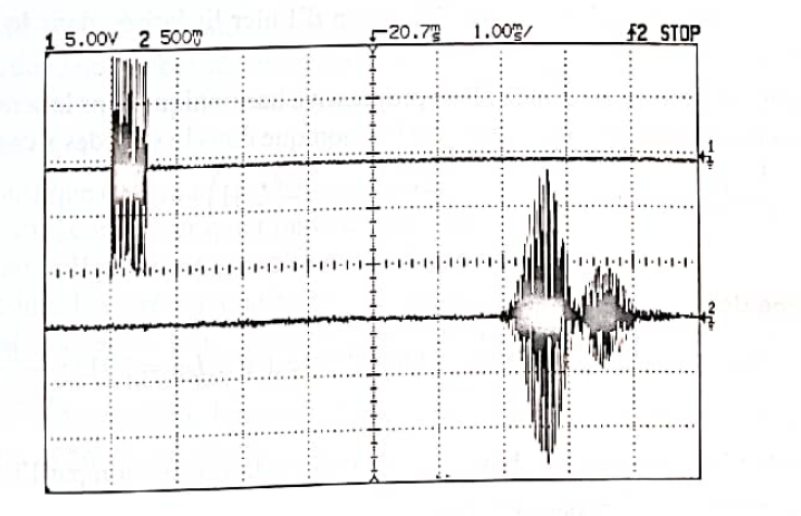
\includegraphics[width=0.4\textwidth]{signal.png}
      \label{fig:signal}
      \caption{Signal sur l'oscilloscope}
    \end{figure}

    L'émetteur est relié à la voie 1 de l’oscilloscope, le récepteur à la voie 2.
  Expliquer le signal observé au niveau du récepteur.
  Mesurer la vitesse de propagation des modes observés.


  \end{itemize}


\end{enumerate}


\end{document}



\section{Exercice 1}

\section{Exercice 2}

\section{Exercice 3}

\section{ Formulaire }

\end{document}